% !TEX spellcheck = en_US
% !TEX spellcheck = LaTeX
\documentclass[a4paper,english,10pt]{article}
\usepackage{%
	amsfonts,%
	amsmath,%	
	etex,%
	amssymb,%
	amsthm,%
	babel,%
	bbm,%
	%biblatex,%
	caption,%
	centernot,%
	color,%
	enumerate,%
	epsfig,%
	epstopdf,%
	geometry,%
	graphicx,%
	hyperref,%
	latexsym,%
	mathtools,%
	multicol,%
	pgf,%
	pgfplots,%
	pgfplotstable,%
	pgfpages,%
	proof,%
	psfrag,%
	subfigure,%	
	tikz,%
	ulem,%
	url%
}	

\usepackage[mathscr]{eucal}
\usepgflibrary{shapes}
\usetikzlibrary{%
  arrows,%
	backgrounds,%
	chains,%
	decorations.pathmorphing,% /pgf/decoration/random steps | erste Graphik
	decorations.text,%
	matrix,%
  	positioning,% wg. " of "
  	fit,%
	patterns,%
  	petri,%
	plotmarks,%
  	scopes,%
	shadows,%
  	shapes.misc,% wg. rounded rectangle
  	shapes.arrows,%
	shapes.callouts,%
  	shapes%
}

\theoremstyle{plain}
\newtheorem{thm}{Theorem}[section]
\newtheorem{lem}[thm]{Lemma}
\newtheorem{prop}[thm]{Proposition}
\newtheorem{cor}[thm]{Corollary}

\theoremstyle{definition}
\newtheorem{defn}[thm]{Definition}
\newtheorem{conj}[thm]{Conjecture}
\newtheorem{exmp}[thm]{Example}
\newtheorem{assum}[thm]{Assumptions}
\newtheorem{axiom}[thm]{Axiom}

\theoremstyle{remark}
\newtheorem{rem}{Remark}
\newtheorem{note}{Note}

\newcommand{\norm}[1]{\left\lVert#1\right\rVert}
\newcommand{\indep}{\!\perp\!\!\!\perp}
\DeclarePairedDelimiter\abs{\lvert}{\rvert}%
%\DeclarePairedDelimiter\norm{\lVert}{\rVert}%
\newcommand{\tr}{\operatorname{tr}}
\newcommand{\R}{\mathbb{R}}
\newcommand{\Q}{\mathbb{Q}}
\newcommand{\N}{\mathbb{N}}
\newcommand{\E}{\mathbb{E}}
\newcommand{\Z}{\mathbb{Z}}
\newcommand{\B}{\mathscr{B}}
\newcommand{\C}{\mathcal{C}}
\newcommand{\T}{\mathscr{T}}
\newcommand{\F}{\mathcal{F}}
\newcommand{\G}{\mathcal{G}}
%\newcommand{\ba}{\begin{align*}}
%\newcommand{\ea}{\end{align*}}

\makeatletter
\def\th@plain{%
  \thm@notefont{}% same as heading font
  \itshape % body font
}
\def\th@definition{%
  \thm@notefont{}% same as heading font
  \normalfont % body font
}
\makeatother
\date{}

%opening
\title{Lecture 04: Compound Poisson Processes}
\author{}
\date{}
\begin{document}
\maketitle

\section{Queueing Theory}
Consider the scenario of a bus stop or a movie ticket counter. Each person arrives to the queue at a random time and has to wait another random amount of time before he is serviced. A natural question to ask is regarding the expected total waiting time of all the people in the queue. To answer this question, we first formalize the idea of a queue.
\subsection{A Preliminary example}
Consider a queue where the customers are arriving according to a Poisson Process $N(t)$ of rate $\lambda$. Recall that $N(t)$ is a random variable that denotes the number of arrivals till time $t$ with $S_n$ the time instant of $n^{\text{th}}$ arrival. 
If $N(t)=n$, then the total expected waiting time is given by
\begin{align}
\label{eqn:WaitingTime}
\E\left[\sum_{i=1}^{N(t)}(t-S_i)\right]=\E\left[\E\left[\sum_{i=1}^{n}(t-S_i)\Big|N(t)=n\right]\right]
\end{align}
Recall that given the number of arrivals in a particular time duration, the arrivals are order statistics of uniformly distributed random variables in that time interval. 
Let $U_1, U_2, \ldots, U_n$ be \emph{iid}  uniform on $[0,t]$, and let $U_{(1)},U_{(2)},\ldots,U_{(n)}$ be their order statistics. 
Then
\begin{align*}
\E\left[\sum_{i=1}^{n}(t-S_i)|N(t)=n\right] &= \E\left[\sum_{i=1}^{n}(t-U_{(i)})\Big| N(t)=n\right]
	= nt-\E\left[\sum_{i=1}^{n}U_i \Big| N(t)=n\right]
	= \frac{nt}{2}.
\end{align*}
Substituting conditional expectation in equation~\ref{eqn:WaitingTime}, we obtain
\begin{align*}
\E\left[\sum_{i=1}^{N(t)}(t-S_i)\right] %&= \E\left[\frac{N(t)t}{2}\right]\\
&= \E\left[N(t)\right]\frac{t}{2} = \frac{\lambda t^2}{2}.
\end{align*}

\subsection{Notations}
\begin{figure}[hhhh]
	\center
	
\begin{tikzpicture}[>=latex]
% the rectangle with vertical rules
\draw (0,0) -- ++(2cm,0) -- ++(0,-1.5cm) -- ++(-2cm,0);
\foreach \i in {1,...,4}
  \draw (2cm-\i*10pt,0) -- +(0,-1.5cm);

% the circle
\draw (2.75,-0.75cm) circle [radius=0.75cm];
\draw (2.75,1.75cm) circle [radius=0.75cm];
\draw (2.75,-3.25cm) circle [radius=0.75cm];
% the arrows and labels
\draw[->] (3.5,-0.75) -- +(20pt,0);
\draw[<-] (0,-0.75) -- +(-20pt,0) node[left] {$\lambda$};
\node[align=center] at (1cm,-2cm) {Buffer};
\node[align=center] at (3cm,-2cm) {Service \\ Node};
\end{tikzpicture}
	\caption{A general queue}
	\label{Fig:queue}
\end{figure}
A queue is denoted as $G_1/G_2/K_1/K_2$
where
\begin{enumerate}
	\item $G_1$ denotes the arrival distribution, %: Memoryless-M, General-G, Deterministic
	\item $G_2$ denotes the service distribution, %: Memoryless-M, General-G, Deterministic
	\item $K_1$ denotes the number of servers,  and%: finite or infinite
	\item $K_2$ denotes the size of the buffer.%: usually infinite and hence omitted in the notation
\end{enumerate}
\begin{rem}
Typical arrival and service distributions are taken to be independent. 
\end{rem}
\begin{rem} Memoryless, general and deterministic distributions are denoted by $M$, $G$, and $D$ respectively. 
\end{rem}
\begin{rem}
Number of servers and buffer sizes can be finite of infinite.
\end{rem}
\begin{rem}
Service policy of the queue could be first in first out (FIFO), last in first out (LIFO), or Processor sharing. 
%We will only consider the First In First Out scenario here.
\end{rem}

\subsection{$M/G/\infty$ Queue}
The $M/G/\infty$ queue has a memoryless arrival distribution with infinite number of servers and a general service distribution $G$. 
Since, this queue has infinite servers, each arriving customer can enter an idle server immediately on arrival. 
We are interested in computing waiting time distribution of any customer in this queue.
To this end, we can diving incoming customers into following two types.
\begin{enumerate}
	\item \textbf{Type-1 customer} whose service is finished by time $t$.
	\item \textbf{Type-2 customer} who doesn't complete the service by time $t$.
\end{enumerate}
%The service distribution $G$ is nothing but
%\begin{align*}
%\Pr\{S_n\leq s\}=G(s)
%\end{align*}
Probability of a customer who arrived at time $s$ and leaves by time $t$ is given by 
\begin{align*}
P(s) &= \Pr\{\text{service time } \leq t  - s \} = G(t-s)\textbf{1}_{\{s\leq t\}}. 
\end{align*}
Let $N_1(t)$ be the number of type-1 customers that arrived in duration $[0,t)$. 
Then
\begin{align*}
\E\left[N_1(t)\right]=p\E\left[N(t)\right],
\end{align*}
where $p=\frac{1}{t}\int_{0}^{t}P(s)ds$.


\subsection{Busy Period of $M/G/1$ Queue}
The $M/G/\infty$ queue has a memoryless arrival distribution with single server and a general service distribution $G$. 
We consider FIFO service policy at the server.
For a queue with single server and FIFO service policy, arriving customer enters the service only if the server is free.
If the server is serving other customer, arriving customers wait in the queue. 
\begin{defn} We define \textbf{busy period} of a queue by the duration when server is busy, and denote it by $B$. It starts when an incoming arrival finds and idle server, and ends when there are no more customers in the system.
\end{defn}

We are interested in characterizing the distribution of busy period $B$, in terms of following system parameters.
We denote rate of Poisson arrival by $\lambda$, and number of customers that arrive in time duration $[0,t)$ by $N(t)$.
%Recall, our notation for $\Pr\{N(t) = n\} = P_n(t)$.
Service times $\{Y_i: i \in \N\}$ of individual customers are assumed \emph{iid} with distribution $G$ and independent of the arrivals.
We denote sum of $k$ service times by $T_k = \sum_{i \in [k]}Y_i$.
Since service time are iid, we can denote distribution of sum of $k$ iid service times by $G_k$, the $k$-fold convolution of $G$.
Without loss of generality, we start the busy period at time $0$ when an arriving customer sees an idle server.
We denote arrival instant of $k^{\text{th}}$ additional customer during a busy period, by $S_k$.%, the time until $k$ additional customers have arrived after time $0$.
% i.e there have been $k$+1 arrivals into the system.
\begin{lem}
\label{Lemma:Equivalence}
Busy period is of duration $t$ and consists of $n$ services if and only if
\begin{enumerate}
	\item $S_k \leq T_k$ for all $k \in [n-1]$,
	\item $T_n=t$,
	\item $N(t)=n-1$.
\end{enumerate}
\end{lem}
\begin{thm}
Distribution of busy period of an $M/G/1$ queue is given by
\begin{align*}
\Pr\{B \leq t\}  = \sum_{n \in \N}\int_{0}^te^{-\lambda u}\frac{(\lambda u)^{n-1}}{n!}dG_n(u).
\end{align*}
\end{thm}
\begin{proof}
%We wish to compute the Probability that the busy period lasts for time t and consists of n services i.e.
From Lemma~\ref{Lemma:Equivalence}, we can write
\begin{align*}
\Pr\left\{B \leq t , N(t) = n-1\right\} 
%& = \Pr\left\{ S_k \leq \sum_{i=1}^{k}Y_i, k \in [n-1], \sum_{i=1}^{n}Y_i=t, N(t)=n-1 \right\}\\
& = \int_{0}^{t}\Pr\left\{ S_k \leq T_k , k\in [n-1] \Big| N(u)=n-1, T_n=u \right\}dG_n(u) P_{n-1}(u) .
%\nonumber\\
%&  \times \underbrace{\Pr\left\{N(t)=n-1, \sum_{i=1}^{n}Y_i=t\right\}}_{dG_n(t) P_{n-1}(t)}
\end{align*}
%where $G_n$ is the n time convolution of the service distribution. Also note that the service distribution of n customers is independent of the value of $N(t)$.
Further, from total probability law, we know that
\begin{align*}
\Pr\{B \leq t\} &=\sum_{n \in \N}\Pr\{B \leq t, N(t)=n-1\}.
\end{align*}
Hence, it suffices to show that $\Pr\{ S_k \leq T_k , k\in [n-1] | N(u)=n-1, T_n=u \} = 1/n$. 
Recall that given $N(u) = n-1$, arrival instants $\{S_k: k \in [n-1]\}$ are order statistics of $n-1$ iid uniform random variables  $\{U_i: i \in [n-1]\}$ in $[0,u)$. 
Clearly, $\{u-U_i: i \in [n-1]\}$ are also iid uniform random variables in $[0,u)$, and order statistics of these random variables would be $\{S_{n-k}: k \in [n-1]\}$.
Then, using Lemma~\ref{Lemma:Final} we can write
\begin{align*}
\Pr\left\{S_k \leq T_k, k \in [n-1]\Big| T_n=u\right\}
&= \Pr\left\{u-S_{n-k} \leq u - (T_n - T_{n-k}),k \in[n-1] \Big| T_n=u\right\}
=\frac{1}{n}.
\end{align*}
%Again in Eq. (2) denote 
%\begin{align*}
%	B(t,n)&=\Pr(\{B=t\}  \cap \{N(B)=n-1\})\\
%&= 	\int_{0}^{t}\frac{1}{n}\times dG_n(t) P_{n-1}(t)\\
%&= \int_{0}^{t}\frac{1}{n}\times dG_n(t)\times \frac{e^{-\lambda t}(\lambda t)^n}{(n-1)!}\\
%\end{align*}
%The distribution of the length of a busy period is then given by
%\begin{align}
%\Pr(B\leq t)=\sum_{n=1}^{\infty}B(t,n)
%\end{align}
\end{proof}

\begin{lem}
\label{Lemma:Uniform}
Let $\{Y_i \geq 0,i \in [n]\}$ be \emph{iid} random variables. 
Then, for all $A \subseteq [n]$, we have
\begin{align*}
 \E\left[\sum_{i \in A}Y_i \Big| \sum_{i \in [n]}Y_i=y\right]=\frac{|A|y}{n}.
\end{align*}
\end{lem}
\begin{proof} Since $Y_i$'s are iid, we notice that
\begin{align*}
y = \E\left[\sum_{i \in [n]}Y_i \Big| \sum_{i \in [n]}Y_i=y\right] = n \E\left[Y_i \Big| \sum_{i \in [n]}Y_i=y\right].
% =  \E\left[\sum_{i \in A}Y_i \Big| \sum_{i \in [n]}Y_i=y\right] +  \E\left[\sum_{i \in A^c}Y_i \Big| \sum_{i \in [n]}Y_i=y\right].
\end{align*}
Hence, we can conclude the result.
%\begin{align*}
%\E\left[\sum_{i \in A}Y_i \Big| \sum_{i \in [n]}Y_i=y\right] & = |A| \E\left[Y_i \Big| \sum_{i \in [n]}Y_i=y\right] = \frac{ky}{n}.
%\end{align*}
\end{proof}

\begin{lem}
\label{Lemma:Reduction}
Let \{$U_i,i \in[n]$\} be iid random variables in $[0,t)$ and $\{U_{(i)},i \in [n]\}$ be their order statistics. Then conditioned on $U_{(n)}=u,\{U_i,i \in[n-1]\}$ are the order statistics of $n-1$ uniform random variables in $[0,u)$.
\end{lem}
\begin{proof}
For order statistics of $n$ uniform random variables in $[0,t)$ and for $u_1 \leq \ldots \leq u_n$, we get
\begin{align*}
\Pr\{U_{(1)} \leq u_1, \ldots, U_{(n)} \leq u_n\} = n!\prod_{i=1}^{n}\frac{u_i}{t}
\end{align*}
Further, distribution of $U_{(n)} = \max_{i \in [n]} U_i$ is given by 
\begin{align*}
\Pr\{U_{(n)} \leq u\} = \left(\frac{u}{t}\right)^n.
\end{align*}
Combining these two results, we get
\begin{align*}
\Pr\{U_{(1)} \leq u_1, \ldots, U_{(n-1)} \leq u_{n-1} | U_{n} = u\} = (n-1)!\prod_{i=1}^{n-1}\frac{u_i}{u}.
\end{align*}
\end{proof}

\begin{lem}
\label{Lemma:CndUniform}
Let $\tau_1,\tau_2,\ldots,\tau_n$ denote the ordered statistics of $n$ iid uniformly distributed random variables in $(0,t)$. Let $\{Y_i,i \in [n]\}$ be iid non-negative random variables independent of $\tau_1,\tau_2,\ldots,\tau_n$. Then for $y \in (0,t)$, we have
\begin{align}
\Pr\left\{\sum_{i\in [k]}Y_i \leq \tau_k,k \in [n] \Big| \sum_{i\in [n]}Y_i=y \right\} = 
1-\frac{y}{t}.
\end{align}
\end{lem}
\begin{proof}
We will prove this by induction on $n$. For base step of $n = 1$, inductive hypothesis is true since
\begin{align*}
\Pr(Y_1 < \tau_1 | Y_1=y) &= \Pr(y < \tau_1).
\end{align*}
We assume the inductive hypothesis to be true for $n-1$. 
Defining $T_k = \sum_{i \in [k]}Y_i$, %we can write
%\begin{align*}
%\Pr\left\{T_k \leq \tau_k,k\in [n] \Big| T_n=y, T_{n-1} = s \right\} 
%& = \int_{0}^{t} \Pr\left\{ T_k \leq \tau_k,k\in [n] \Big| T_n = y, T_{n-1} = s, \tau_n = u\right\} d\Pr\{\tau_n \leq u\}.
%% | T_n=y,T_{n-1}=s\}.
%\end{align*}
%Using the Lemma~\ref{Lemma:Reduction}, we can write the integrand for $ y \in (0,u)$ as 
and using Lemma~\ref{Lemma:Reduction}, we can write
\begin{align*}
\Pr\left\{ T_k \leq \tau_k,k\in [n] \Big| T_n = y, T_{n-1} = s, \tau_n = u \right\}= 
%\begin{cases}
\Pr\left\{T_k \leq \tau_k^{\ast},k \in [n-1] \Big| T_{n-1}=s \right\}.
%& y < u\\.
%0 & y \geq u.
%\end{cases}
\end{align*}
where $\tau_k^*$ are order statistics of $n-1$ iid uniform random variables in $[0,u)$. 
From inductive hypothesis, it follows that %for $y \in [0,u)$, we have
%From Lemma \ref{unif}
%\begin{align*}
%\Rightarrow  \Pr(*) = 
%\begin{cases}
%1-\frac{s}{u} & y < u\\
%0 & y \geq u.
%\end{cases}
%\end{align*}
\begin{align*}
\Pr\left\{T_k \leq \tau_k,k\in [n] \Big| T_n, T_{n-1}, \tau_n \right\}=
%\begin{cases}
\left(1-\frac{T_{n-1}}{\tau_n}\right)1_{\{T_n < \tau_n\}}.%,\\
%0, & y \geq u.
%\end{cases}
\end{align*}
Using Lemma~\ref{Lemma:Uniform}, we can write
\begin{align*}
\Pr\left\{T_k \leq \tau_k, k\in [n] \Big| T_n,  \tau_n\right\} &= \E\left[\left(1-\frac{T_{n-1}}{\tau_n} \right)1_{\{T_n \leq \tau_n\}}\Big| T_n, \tau_n\right]
%\\& = 1-\frac{1}{u}\E\left[\sum_{i=1}^{n-1}Y_i \Big| \sum_{i=1}^{n}Y_i=y\right] 
= \left(1-\frac{(n-1)T_n}{n\tau_n}\right)1_{\{T_n \leq \tau_n\}}.
\end{align*}
Since $\tau_n$ is maximum of $n$ uniform random variables distributed on $[0,t)$, we can write
\begin{align*}
\Pr\{\tau_n \leq x\} &= \left(\frac{x}{t}\right)^n, \text{ for } x \in [0, t).
\end{align*}
Hence, by taking expectation with respect to $\tau_n$, we can write
\begin{align*}
\Pr\left\{T_k \leq \tau_k ,k\in [n] \Big| T_n \right\} %&= \E\left[1-\frac{n-1}{n}\frac{T_n}{\tau_n}\Big| T_n<\tau_n\right]\Pr\{ T_n<\tau_n\}\\
&= \Pr\{ T_n \leq \tau_n\} -\frac{n-1}{n}T_n\E\left[\frac{1}{\tau_n}1_{\{T_n \leq \tau_n\}}\right]\\
&= 1 - \left(\frac{T_n}{t}\right)^n - (n-1)T_n\int_{T_n}^{t}\frac{x^{n-2}}{t^n}dx = 1 - \frac{T_n}{t}.
\end{align*}
%Therefore
%\begin{align*}
%	\E\left[\frac{1}{\tau_n}\Big| \tau_n>y\right]\Pr\{\tau_n>y\}&=\\
%	&=\frac{n}{n-1}\left(\frac{t^{n-1}-y^{n-1}}{t^n}\right)
%\end{align*}
%Hence
%\begin{align*}
%	\Pr\left\{\sum_{i\in [k]}Y_i &\leq \tau_k ,k\in [n] \Big| \sum_{i\in [n]}Y_i=y \right\}\\
%	&= 1-\left(\frac{y}{t}\right)^n-\frac{yt^{n-1}-y^{n-1}}{t^n}\\
%	&= 1-\frac{y}{t}
%\end{align*}
\end{proof}

\begin{lem}
\label{Lemma:Final}
Let $\tau_1, \tau_2, \ldots, \tau_{n-1}$ be the order statistics of $n-1$ \emph{iid} random variables distributed uniformly in $[0,t)$. Let $\{Y_i,i\in [n]\}$	be \emph{iid} nonnegative random variables that are also independent of $\tau_1, \tau_2, \ldots, \tau_{n-1}$. Then
\begin{align*}
\Pr(\sum_{i \in [k]}Y_i < \tau_k,k \in [n-1] |\sum_{i \in [n]}Y_i=t)=\frac{1}{n}
\end{align*}
\end{lem}
\begin{proof} Using definition of $T_k = \sum_{i \in [k]}Y_i$ and Lemma~\ref{Lemma:CndUniform}, we can write
\begin{align*}
\Pr\left\{ T_k<\tau_k ,k \in [n-1] \Big| T_n=t, T_{n-1} \right\}
&= \Pr\left\{T_k<\tau_k,k \in [n-1] \Big| T_{n-1}\right\}=\left(1-\frac{T_{n-1}}{t}\right) \textbf{1}_{\{T_{n-1} < t\}}.
\end{align*}
Hence using Lemma~\ref{Lemma:Uniform}, we have
\begin{align*}
\Pr\left\{T_k<\tau_k,k \in [n-1] \Big| T_n=t\right\} &= \E\left[\left(1-\frac{T_{n-1}}{t}\right) \textbf{1}_{\{T_{n-1} < t\}} \Big|T_n=t\right] = 1-\frac{(n-1)t}{nt} =\frac{1}{n}.
\end{align*}
\end{proof}

\section{Compound Poisson Process}
\begin{defn}
A stochastic Process $\{Z_t,t \geqslant 0\}	$ is said to be a compound Poisson Process if it can be represented as $Z_t=\sum_{i=1}^{N_t}X_i$ for all $t\geq 0$ where $\{N_t,t\geq 0\}$ is a Poisson Process and $\{X_i, i\in \N\}$ are \emph{iid} random variables independent of $\{N_t, t\geq 0\}$.
\end{defn}
Alternately it can also be defined in the following way.
\begin{defn}
A compound Poisson Process is a point Process \{$Z_t,t \geq 0$\} having the following properties.
\begin{enumerate}
	\item For all $\omega \in \Omega, t \longmapsto Z_t(\omega)$ has finitely many jumps in finite intervals.
	\item For all $t,s \geq 0; Z_{t+s}-Z_t$ is independent of $\{Z_u, u\leq t\}$.
	\item For all $t,s \geq 0$, distribution of $Z_{t+s}-Z_t$ depends only on $s$ and not on $t$.
\end{enumerate}	
\end{defn}
\begin{defn} A compound Poisson Process is stationary and independent increments point Process with jump points $S_n=\inf \{t>0 | N(t)=n\}$, and associated jump sizes $X_n$ independent of jump instants.% are the jump sizes associated with the Process.
\end{defn}

\subsection{Examples}
\begin{exmp} Arrival of customers in a store is a Poison Process $N_t
$. Let the amount spent by each customer be \emph{iid} random variables independent of the arrival Process. Amount of money spent by first $n$ customers is
\begin{xalignat*}{3}
&Y_n=\sum_{i=1}^{n}X_i, i \in [n],&&Y_0=0.
\end{xalignat*}
Now define $Z_t=Y_{N_t}$ as the amount spent by the customers arriving in time $t$. Then $\{Z_t,t\geq 0\}$ is a compound Poisson Process.
\end{exmp}

\begin{exmp}  Let the time between successive failures of a machine be independent and  exponentially distributed. The cost of repair is \emph{iid} random at each failure. Then the total cost of repair in a certain time t is a compound Poisson Process.
\end{exmp}

\begin{exmp}  Let $X_i\in E$ where $E$ is a countable set. Let $N_t^e$  be the number of jumps of size $e$ in time $[0,t)$.
\begin{rem} Observe that $\{N_t^e, e\in E\}$ are independent Poisson with rate \{$\lambda_e: e\in E$\}  where $\lambda_e=\lambda \Pr\{X_i=e\}$.
\end{rem}
We define $Z_t=\sum_{e\in E}eN_t^e$, to obtain
\begin{align}\label{obs}
\E\left[e^{-\theta Z_t}\right]=\E\left[\prod_{e\in E}e^{-\theta e N_t^e}\right]=\prod_{e\in E}\E\left[e^{-\theta e N_t^e}\right]
\end{align}
However, we have
\begin{align*}
\E\left[e^{-\theta N_t}\right] &= \sum_{n=0}^{\infty}e^{-\theta n}e^{-\lambda t}\frac{(\lambda t)^n}{n!} 
%= e^{-\lambda t} e^{\lambda te^{-\theta}}
= e^{-\lambda t(1-e^{-\theta})}.
\end{align*}
Substituting this back in equation~\eqref{obs}, we obtain
\begin{align*}
\E\left[e^{-\theta Z_t}\right] &= \prod_{e\in E}e^{-\lambda_et(1-e^{-\theta e})}\\
&= \exp\left[-t\sum_{e\in E}\lambda(1-e^{-\theta e})\Pr\{X_i=e\}\right]
\end{align*}
\end{exmp}

\begin{exmp} If $X_i$ \emph{iid} with mean $\mu$, then we can find mean off $Z_t$ as
\begin{align*}
 \E\left[Z_t\right] = \E\left[\E[Z_t|N_t]\right]&=\E\left[\E\left[\sum_{i=1}^{N_t}X_i|N_t\right]\right] = \mu\E N_t = \lambda \mu t.
\end{align*}
\end{exmp}

\begin{exmp}  If $X_i$ are \emph{iid} with a distribution function $\varphi$, then we can write moment generating function of $Z_t$ in terms of moment generating function $f(\theta) = E[e^{-\theta X_1}]$ of $X_1$ as
\begin{align*}
\E\left[e^{-\theta Z_t}\right] &= \E\left[\E\left[e^{-\theta\sum_{i=1}^{n-1}X_i}\right]\big|N_t\right] 
%= \sum_{n=0}^{\infty}P_n(t)f(\theta)^n\\
= \sum_{n=0}^{\infty}e^{\lambda t}\frac{(-\lambda t)^n}{n!}f(\theta)^n
%&= e^{-\lambda t}e^{\lambda t f(\theta)}\\
= e^{-\lambda t (1-f(\theta))}\\
&= \exp\left[-t\int_{0}^{\infty}(1-e^{-\theta u})\lambda d\varphi(u)\right].
\end{align*}
\end{exmp}

%\section{Compound Poisson Process}
%One of the characterizations of Poisson Process was single arrival in an infinitesimal time. We can generalize that definition to have a random number of arrivals $X_n$ at every arrival instant $S_n$.
%\begin{defn}[Compound Poisson Process] Let $\left\{X_i\right\}$ be \emph{iid} random variables. Let $N(t), t\geq 0$ be a Poisson Process with parameter $\lambda$ independent of $X_i, i\geq 1$. Then the Process $X(t)$ defined as
%	\begin{align*}
%		X(t) = \sum_{i=1}^{N(t)} X_i
%	\end{align*}
%	is called a \textbf{compound Poisson Process}.
%\end{defn}
%\subsection{properties of the compound Poisson Process}
%\subsubsection{Mean}
%\begin{align*}
%	E[X(t)] = E[\sum_{i=1}^{N(t)} X_i] &= E[E[\sum_{i=1}^{N(t)} X_i|N(t)]] \\
%	&= \sum_{k=0}^\infty E\left[\sum_{i=1}^{k} X_i|N(t)=k\right]\Pr\{N(t) = k\}\\
%	&= \sum_{k=0}^\infty \sum_{i=1}^{k} E[X_i]\Pr\{N(t) = k\}\\
%	&= E[N(t)]E[X_1] = \lambda tE[X_1].
%\end{align*}
%
%\subsubsection{MGF}
%We leave it as an exercise to show that $M_{X(t)}(\theta)=E[e^{\theta X(t)}] = e^{(M_X(\theta)-1)\lambda t}$.

\subsubsection{A nice counterexample}
A Poisson Process is not uniquely determined by it's distribution. Let $X_t = Y_t + f(Z+t)$, where $Y_t$ is a Poisson Process and 
\begin{align*}
	f(t) = t 1_{\{t \in \mathbb{Q}\}}.
\end{align*}
Let $Z$ be a continuous random variable. Then we can show that $\Pr\{X_t \neq Y_t) = 0$. This is true since
\begin{flalign*}
	\Pr\{X_t \neq Y_t\} &= \Pr\{\omega \in \Omega: \quad t+Z(\omega) \in \mathbb{Q}\} \\
	&= \Pr\{\omega \in \Omega:  Z(\omega) \in \mathbb{Q} - t\} = 0.
\end{flalign*}
The last part follows since $\mathbb{Q}-t$ is a countable set of individual events with Probability zero. We can also show that $X(t)$ and $Y(t)$ have same fdds.
\begin{align*}
	\Pr\{X_{t_1}= Y_{t_1}, X_{t_2}= Y_{t_2}\}
	= \sum_{n_{1},n_{2}}\Pr\{X_{t_1} = n_1, X_{t_2}= n_2, Y_{t_1}=n_1, Y_{t_2}=n_2 \}  = 1.
\end{align*}
$\{X_{t}(\omega)\}$ can take non-integer values and is not non-decreasing. Two Process can have same distribution but sample path behavior can be quite different.
%\section{Compound (Batch) Poisson Process}
%
%\begin{eqnarray*}
%% \nonumber to remove numbering (before each align)
%N_{t} &=& \sup \{n: S_{n}\leq t \}  \\
%\end{eqnarray*}
%$\overline{N_{t}}$= No of arrivals till time $n$  \\
%\begin{eqnarray*}
%\overline{N_{t}}&=& \sum ^{N_{t}}_{k=0}Z_{k}  ~(\text{No. of arrivals till time $n$}).\\
%\E[\overline{N_{t}}]&=&\E\left[\sum ^{N_{t}}_{k=0}Z_{k}\right]  \\
%&=& \sum^{\infty}_{n=0}\E\left[\sum ^{N_{t}}_{k=0}Z_{k}|N_{t}-n \right] P[N_{t}=n]\\
%&=& \sum^{\infty}_{n=0}P[N_{t}=n]\E\left[\sum^{\infty}_{k=0}Z_{k}|N_{t}=n   \right] \\
%&=& \sum^{\infty}_{n=0} \frac{e^{-\lambda t} (\lambda t)^{n}}{n!} n \E[Z_{1}] \\
%&=& \E [Z_{1}]\E [N_{t}].
%\end{eqnarray*}
%For  $  \alpha>0 $,  \\
%\begin{eqnarray*}
%&\E[e^{\alpha \overline{N_{t}}}]=\E\left[e^{\alpha\sum ^{N_{t}}_{k=0}Z_{k}}\right] \\
%&=& \sum^{\infty}_{n=0}\E\left[ e^{\alpha\sum ^{N_{t}}_{k=0}Z_{k}}| N_{t}=n\right] P[N_{t}=n]\\
%&=&  \sum^{\infty}_{n=0}\E\left[e^{\alpha\sum ^{n}_{k=0}Z_{k}}\right] P[N_{t}=n]\\
%&=&\E[\E[e^{\alpha Z_{1}}]^{N_{t}}]\\
%\E [\beta^{N_{t}}] &=&\sum^{\infty}_{n=0}\frac{(\lambda t)^{n}e^{-\lambda t}}{n!}\beta^{n}\\
%&=&\sum^{\infty}_{n=0}\frac{(\lambda \beta t)^{n}e^{-\lambda \beta t}}{n!}\lambda (\beta t-t)\\
%&=& e^{\lambda t (\beta-t)}
%\end{eqnarray*}
%\textbf{Example:}\\
%\begin{figure}[h!]
%\center
%% Requires \usepackage{graphicx}
%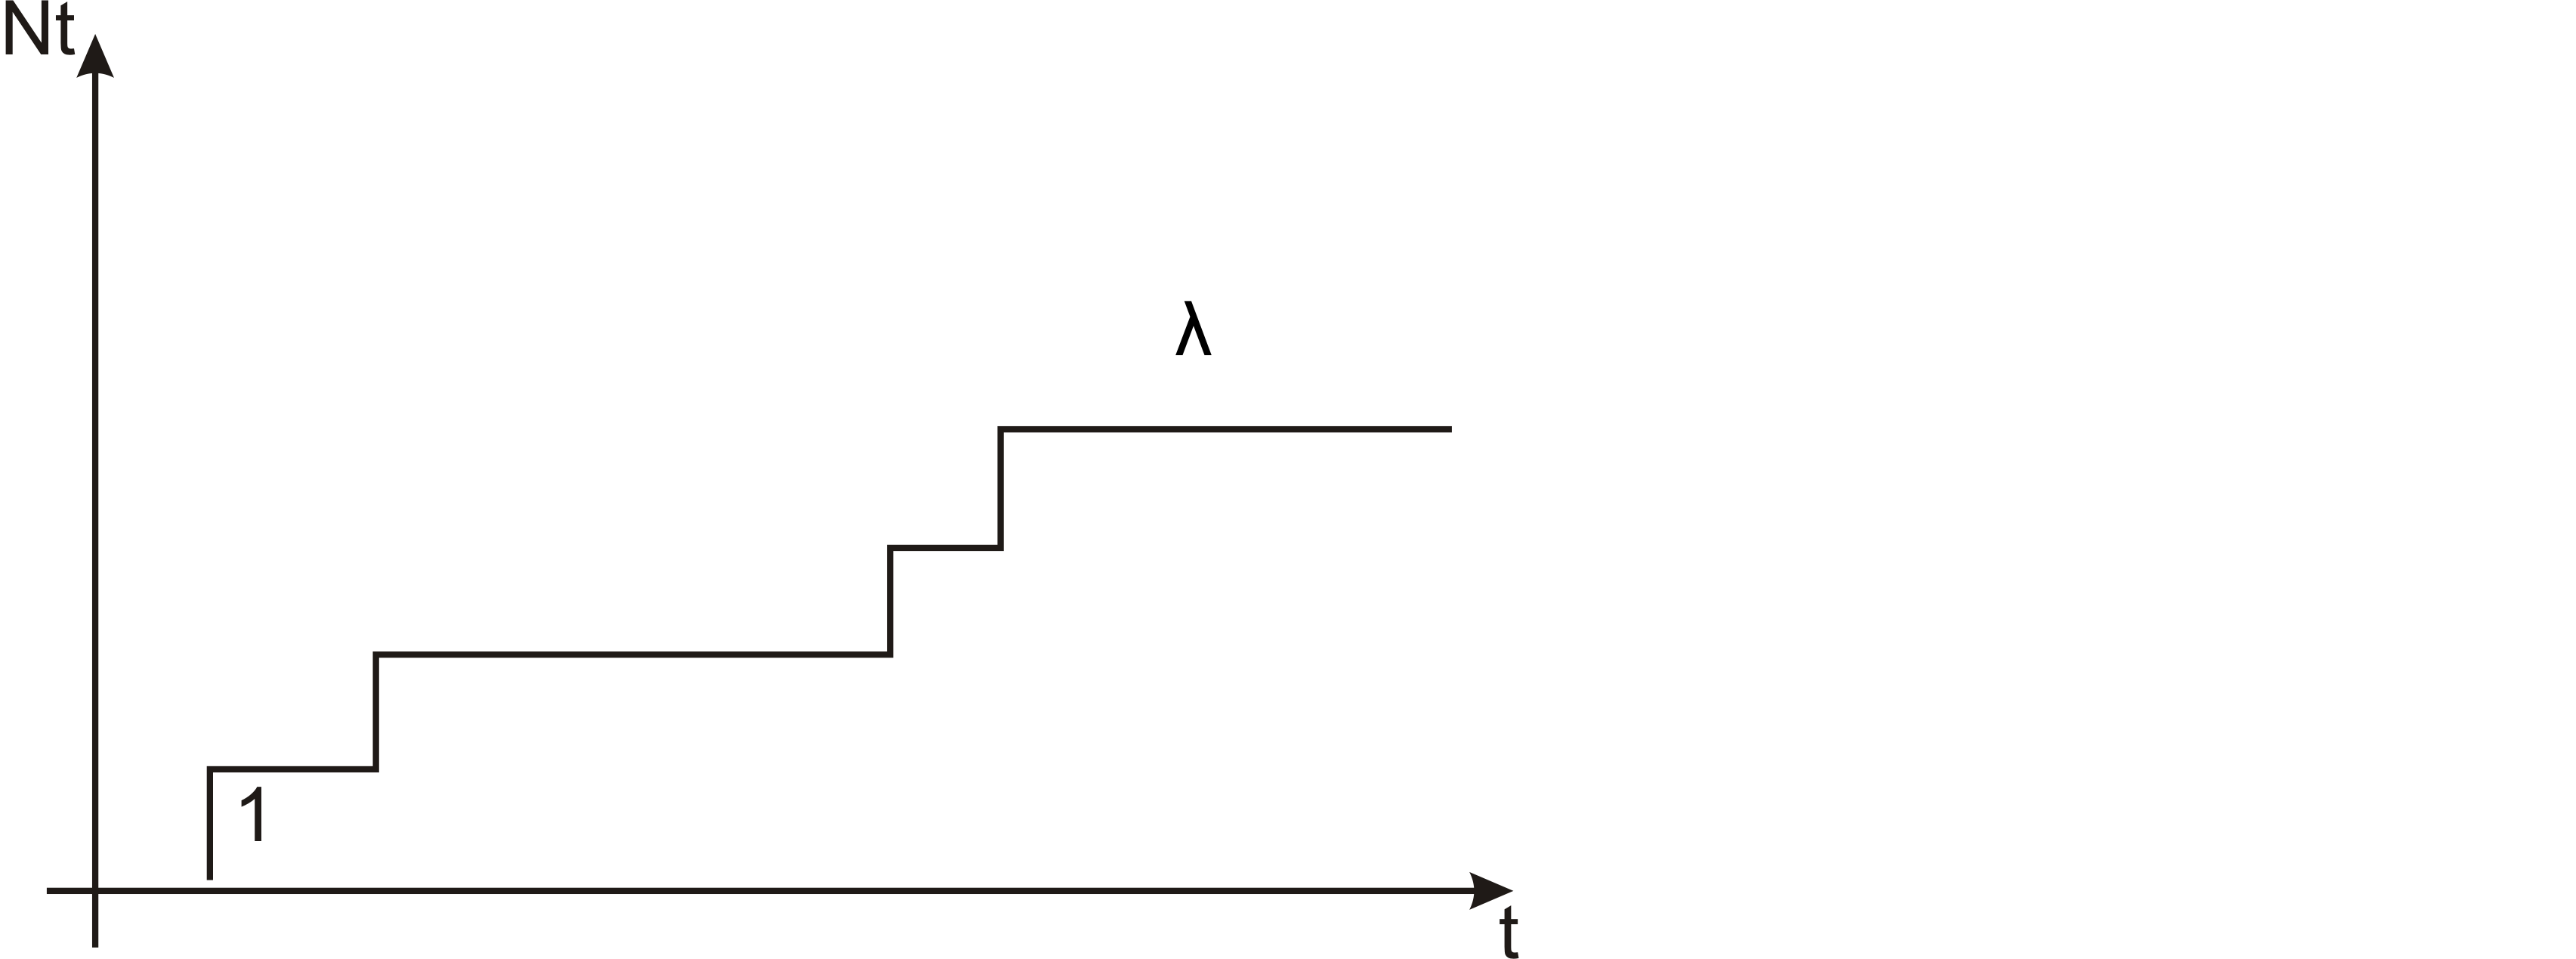
\includegraphics[width=4.5in]{Figures/rate.PNG}\\
%% \caption{}\label{}
%\end{figure}
%Suppose $\{N_{t}, t \geq 0\}$ Poisson Process with rate $\lambda$. 
%
%$\tilde{N_{t}}(w)= N_{t}(w)+f(t+X_{1}(w))$ where $f(t)$=0, if $t$ is irrational and $f(t)$=t, if $t$ is rational.\\
%\begin{eqnarray*}
%% \nonumber to remove numbering (before each align)
%P[\tilde{N_{t}}\neq N_{t}] &= P[\omega:t+X_{1}(\omega) \text{is rational}],\\
%&= P[\omega:X_1(\omega)  \text{is rational} ] =0.
%\end{eqnarray*}


\section{Non-Homogeneous Poisson Process}
From the characterization of Poisson Process just stated, we can generalize to non-homogeneous Poisson Process. In this case, the rate of Poisson Process $\lambda$ is time varying. It is not clear from the first two characterizations, how to generalize the definition of Poisson Process to the non-homogeneous case. We used third characterization of Poisson Process for this generalization. 

\begin{defn}[Non-Homogeneous Poisson Process]\label{defn:NonHomogeneousPoisson} A point Process $\{N(t),~t\geqslant 0\}$ is said to be \textbf{non-homogeneous Poisson Process} with instantaneous rate $m(t)$ if it has stationary independent increments, and 
	\begin{eqnarray*}\label{eq:NonHomogeneousPoisson}
		\Pr\{N(t)=0\}&=&1-m(t)+o(t). \\
		\Pr\{N(t+\delta)-N(t)=0\} &=& 1-m(t)\delta+o(\delta). \\
		\Pr\{N(t+\delta)-N(t)=1\} &=& m(t)\delta+o(\delta). \\
		\Pr\{N(t+\delta)-N(t)>1\} &=& o(\delta). \\
	\end{eqnarray*}
\end{defn}

\begin{prop}[Non-Homogeneous Distribution] Distribution of non-homogeneous Poisson Process $N(t)$ with instantaneous rate $m(t)$ is given by
	\begin{align*}
		\Pr\{N(t)=n\}=\frac{(\bar{m}(t))^n}{n!}e^{-\bar{m}(t)},
	\end{align*}
	where $\bar{m}(t)$ is the cumulative rate till time $t$, i.e. $\bar{m}(t)=\int_{0}^{t}m(s)ds$. 
\end{prop}
\begin{proof}
	Let's denote $f(t) = \Pr\{N(t)=0\}$. Further, from independent increment property of $N(t)$, we notice that $\{N(t+\delta) = 0\}$ is intersection of two independent events given below, 
	\begin{align*}
		\{N(t+\delta)=0\} \iff \{N(t)=0\}\cap\{N(t+\delta)-N(t)=0\}.
	\end{align*}
	From Definition~\ref{defn:NonHomogeneousPoisson}, it follows that
	\begin{align*}
		f(t+\delta) = f(t)[1 - m(t)\delta + o(\delta)].
	\end{align*}
	Re-arranging the terms in the above align, dividing by $\delta$, and taking limit as $\delta \downarrow 0$, we get 
	\begin{align*}
		f'(t) = -m(t)f(t).
	\end{align*}
	Since $f(0) = 1$, it can be verified that $f(t) = \exp(-\bar{m}(t))$ is solution for $f(t)$.
	%\begin{eqnarray*}
	%f(t+\triangle) &=& \Pr\{N_{t+\triangle}=0] \\
	%&=&  \Pr\{N(t)=0, N_{t+\triangle}-N(t)=0]\\
	%&\stackrel{(a)}{=}& \Pr\{N(t)=0] \Pr\{N_{t+\triangle}-N(t)=0]\\
	%&=& f(t)[1-m(t)\triangle +o(\triangle)].\\
	%\frac{f(t+\triangle)-f(t)}{\triangle} &=& -m(t) f(t) +f(t) \frac{0(\triangle)}{\triangle}. \\
	%\lim_{\triangle\downarrow 0}\frac{f(t+\triangle)-f(t)}{\triangle} &=& -m(t) f(t) \\
	%\frac{d f(t)}{t} &=& -m(t) f(t),  \\
	%\end{eqnarray*}
	%where (a) follows from independent increment property. Since, $\overline{m}(t)=\int ^{t}_{0} m(s) ds $, $f(t)=\Pr\{N(t)=0]$, $ f(0)=\Pr\{N_{0}=0] =1$ the solution of the differential align can be verified to be $f(t)=e^{-\overline{m}(t)}$, as follows: 
	%\begin{eqnarray*}
	%f(0)&=& e^{-\overline{m}(t)}\\
	%&=& e^{-0}=1 \\
	%f'(t) &=& e^{-\overline{m}(t)}\frac{d}{dt} \int^{t}_{0}m(S) ds\\
	%&=& m(t)e^{-\overline{m}(t)}, t\geqslant 0 \\
	%\end{eqnarray*}
	%
	%\begin{eqnarray*}
	%\Pr\{N_{t+\triangle}-N(t)=0] &=& 1-m(t)\triangle +o(\triangle) \\
	%\Pr\{N_{\triangle}-N_{0}=0] &=& 1-m(0)\triangle +o(\triangle) 
	%\end{eqnarray*}
	%Since $ N_{0}=0$, 
	%\begin{eqnarray*}
	%\Pr\{N_{\triangle} =0]&=& 1-m(0)\triangle +0(\triangle) \\
	%\lim_{\triangle\downarrow 0}f(\triangle) &=& f(0)=1.
	%\end{eqnarray*}
	We have shown $\Pr\{N(t)=0\} = \exp(-\bar{m}(t))$. By induction, we can show the result for any $n$.
\end{proof}

\end{document}